\documentclass[t]{beamer}


\usepackage{header100}
\usepackage{header_maps}
\usepackage[utf8]{inputenc}


\usepackage{amsfonts}
\usepackage{amssymb}
\usepackage{amsmath}
\usepackage{times}
\usepackage{graphicx}
\usepackage{sidecap}
\usepackage{mathtools}
\usepackage{caption}
\usepackage{breakurl}
\usepackage{bm}
\usepackage[all]{xy}
\usepackage{lipsum}
\usepackage{amsthm}
\usepackage{tikz}
\usepackage{booktabs}
\usepackage{pgfplots}
\usepackage{tabularx}
\usetikzlibrary{positioning}
\usepackage{xurl}
\usepackage{animate}
\usetikzlibrary{shapes,snakes}



\DeclarePairedDelimiter\ceil{\lceil}{\rceil}
\DeclarePairedDelimiter\floor{\lfloor}{\rfloor}

\DeclareMathOperator{\cok}{coker}
\DeclareMathOperator{\im}{im}
\DeclareMathOperator{\ann}{Ann}
\DeclareMathOperator{\Hom}{Hom}

\newcommand{\vv}{\vspace{0.3cm}}

\makeatletter
\newenvironment<>{proofs}[1][\proofname]{%
 \par
 \def\insertproofname{#1\@addpunct{.}}%
 \usebeamertemplate{proof begin}#2}
 {\usebeamertemplate{proof end}}
\makeatother

\newcommand{\ik}[1]{\begin{block}{iClicker Activity} #1 \end{block}}
\newcommand{\ex}[1]{\begin{block}{Exercise} #1 \end{block}}
\newcommand{\co}[1]{[#1)}
\newcommand{\oc}[1]{(#1]}
\newcommand{\p}{\pause}
\newcommand{\ddx}{\frac{d}{dx}}
\newcommand{\eb}[1]{\begin{exampleblock}{} #1 \end{exampleblock}}
\newcommand{\RR}{\mathbb{R}}
\newcommand{\ZZ}{\mathbb{Z}}

\newcommand{\KP}[1]{%
  \begin{tikzpicture}[baseline=-\dimexpr\fontdimen22\textfont2\relax]
  #1
  \end{tikzpicture}%
}
\newcommand{\KPA}{%
  \KP{\filldraw[color=gray, fill=none, thick] circle (0.3);}%
}

\newcommand{\KPUNLINK}{%
  \KP{\filldraw[color=gray, fill=none, thick] circle (0.3);
  \filldraw[color=gray, fill=none, thick] (0.7,0) circle (0.3);}%
}

\newcommand{\KPB}{%
  \KP{
 \draw[color=gray,thick] (-0.3,0.3) -- (0.3,-0.3);
 \draw[color=gray,thick] (-0.3,-0.3) -- (-0.05,-0.05);
 \draw[color=gray,thick] (0.05,0.05) -- (0.3,0.3);
  }%
}

\newcommand{\KPBB}{%
  \KP{
 \draw[color=gray,thick] (-0.3,-0.3) -- (0.3,0.3);
 \draw[color=gray,thick] (-0.3,0.3) -- (-0.05,0.05);
 \draw[color=gray,thick] (0.05,-0.05) -- (0.3,-0.3);
  }%
}

\newcommand{\KPC}{%
  \KP{%
 \draw[color=gray,thick] (-0.3,0.3) .. controls (0,-0.05) .. (0.3,0.3);
 \draw[color=gray,thick] (-0.3,-0.3) .. controls (0,0.05) .. (0.3,-0.3);
  }%
}
\newcommand{\KPD}{%
  \KP{%
 \draw[color=gray,thick] (-0.3,-0.3) .. controls (0.05,0) .. (-0.3,0.3);
 \draw[color=gray,thick] (0.3,-0.3) .. controls (-0.05,0) .. (0.3,0.3);
  }%
}

\newcommand{\knotlinewidth}{.7pt}
\newcommand{\myarrow}{$\quad\longleftrightarrow\quad$}
\newcommand{\RIa}[1][]{\tikz[knot, #1]{\draw(-.5,.5) to[out=-90,in=-90] (.5,0); \draw[overcross] (.5,0) to[out=90,in=90] (-.5,-.5);}}
\newcommand{\RIb}[1][]{\tikz[knot, #1]{\draw[looseness=.8] (-.5,-.5) to[out=90, in=-90] (.5,0) to[out=90, in=-90] (-.5,.5);}}
\newcommand{\RIIa}[1][]{\tikz[knot, #1]{\draw[red, looseness=2.3] (-.5,-.5) to[out=0, in=0] (-.5,.5); \draw[looseness=2.3, overcross=blue] (.5,-.5) to[out=180, in=180] (.5,.5);}}
\newcommand{\RIIb}[1][]{\tikz[knot, #1]{\draw[red, looseness=1.4] (-.5,-.5) to[out=0, in=0] (-.5,.5);\draw[blue, looseness=1.4] (.5,.5) to[out=180,in=180] (.5,-.5);}}
\newcommand{\RIIc}[1][]{\tikz[knot, #1]{\draw[blue, looseness=2.3] (.5,-.5) to[out=180, in=180] (.5,.5); \draw[looseness=2.3, overcross=red] (-.5,-.5) to[out=0,in=0] (-.5,.5);}}
\newcommand{\RIIIa}[1][]{\tikz[knot, #1]{\draw[red] (-120:.58) to[out=60,in=-120] (150:.2) to[out=60, in=-120] (60:.58); \draw[rotate=-120, overcross=blue] (-120:.58) to[out=60, in=-120] (150:.2) to[out=60, in=-120] (60:.58); \draw[rotate=120, overcross=green!80!black] (-120:.58) to[out=60, in=-120] (150:.2) to[out=60, in=-120] (60:.58);}}


\tikzset{overcross/.style={double, line width=1.5, white, double=#1, double distance=\knotlinewidth},
 overcross/.default={black},
 knot/.style={line width=\knotlinewidth, baseline=-.5ex}}

%Information to be included in the title page:
\title{A Layman's Introduction to Knots and Jones Polynomials}
\institute{University of Manitoba}
\author{Junyu Lu}
\date{Nov 2023}
\titlegraphic{
\includegraphics[height=1cm]{pic/um.png}}

\begin{document}

\frame{\titlepage}

\begin{frame}[c]
	\frametitle{Definitions}
	\begin{center}
		Knot = A piece-wise linear (or smooth) embedding of $S^1$ into $\RR^3$ or $S^3$\\
		\vspace{0.1in}
		Link = A p.l. (or smooth) embedding of disjoint circles into $\RR^3$ or $S^3$
	\end{center}
	\p
	\begin{figure}
		\centering
		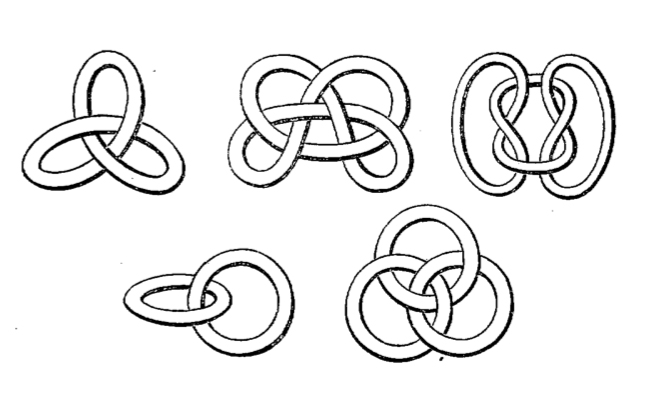
\includegraphics[width=6cm]{pic/kelvin_knots.jpg}
		\caption{Illustrations of knots and links, including a trefoil knot, top left, in an 1869 paper by Lord Kelvin on his knotted vortex theory of atoms.}
	\end{figure}
\end{frame}

\begin{frame}[c]
	\frametitle{Knot Equivalence}
	Two knots are \emph{equivalent} if one knot can be pushed about smoothly, without intersecting itself, to coincide with another knot.

	% \begin{figure}
	%  \centering
	%  \animategraphics[loop,controls,width=4cm]{10}{pic/Knot_Unfolding-}{0}{50}
	%  \caption{Deformation to an unknot}
	% \end{figure}


	\begin{center}
		unknot = the boundary of a simplicial disk
	\end{center}

	%Or more rigorously, defined by ambient isotopy or equivalently by an orientation-preserving homeomorphism of $S^3$ to itself

\end{frame}

\begin{frame}
	\frametitle{Reidemeister Moves}
	\begin{theorem}[Reidemeister 1927]
		Two knots are equivalent if and only if all their diagrams are connected by a finite sequence of Reidemeister moves of Type I, II or III.
	\end{theorem}
	In this case, we also say their diagrams are equivalent.
	% \begin{figure}
	% 	\centering
	% 	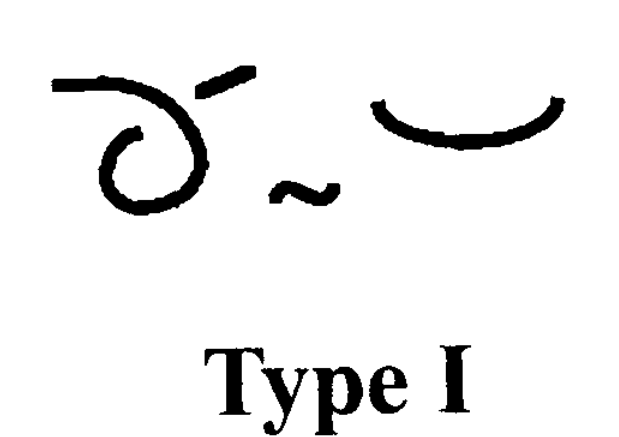
\includegraphics[width=0.22\textwidth]{pic/type1.png}
	% 	\hspace{0.5cm}
	% 	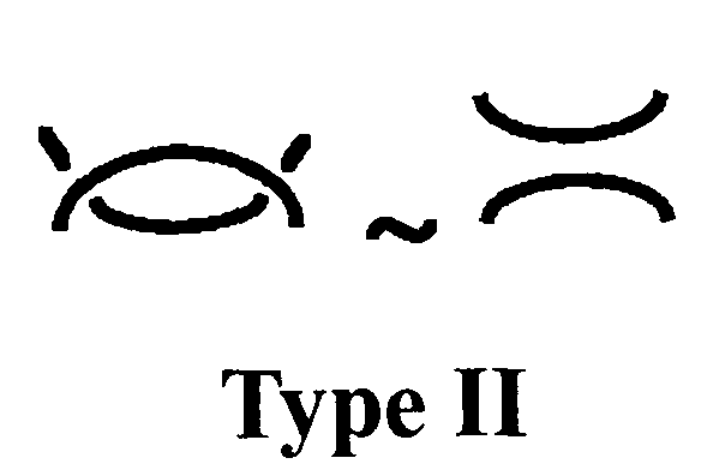
\includegraphics[width=0.24\textwidth]{pic/type2.png}
	% 	\hspace{0.5cm}
	% 	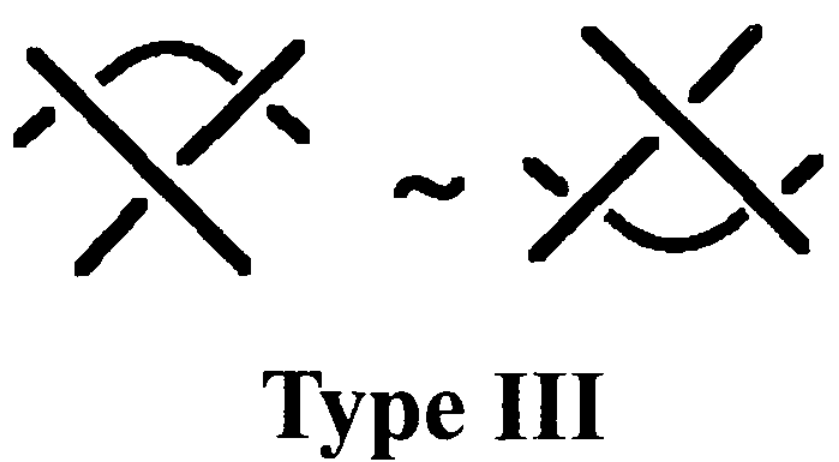
\includegraphics[width=0.24\textwidth]{pic/type3.png}
	% 	\caption{Reidemeister moves}
	% \end{figure}
	\begin{enumerate}[I.]
		\item \RIa\myarrow\RIb
		\item \RIIa\myarrow\RIIb
		\item \RIIIa\myarrow\RIIIa[rotate=180]
	\end{enumerate}
\end{frame}

\begin{frame}
	\frametitle{Reidemeister Moves}
	\begin{block}{Remark}
		The following moves can be seen (exercise) to be consequences of the three types of Reidemeister move.
	\end{block}
	% \begin{figure}
	% 	\centering
	% 	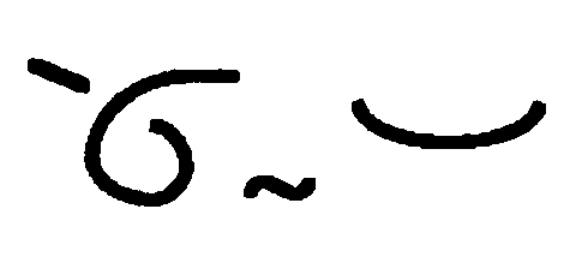
\includegraphics[width=0.22\textwidth]{pic/type11.png}
	% 	\hspace{0.5cm}
	% 	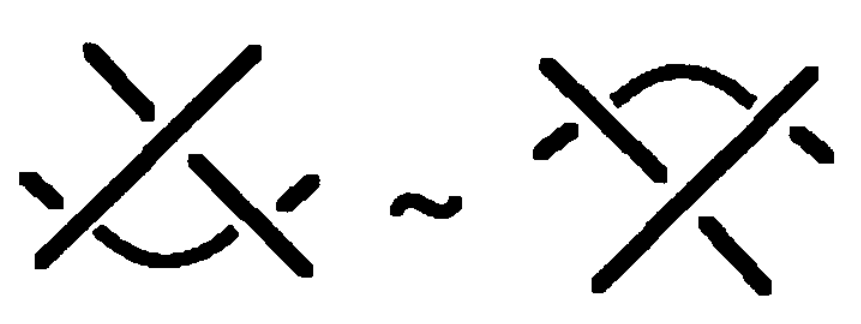
\includegraphics[width=0.24\textwidth]{pic/type21.png}
	% 	\hspace{0.5cm}
	% 	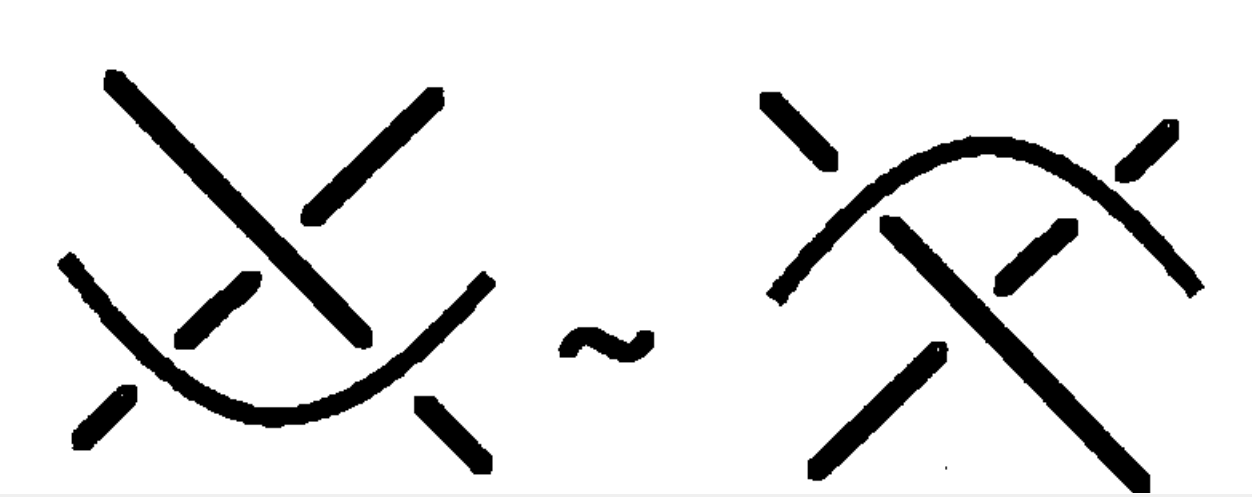
\includegraphics[width=0.24\textwidth]{pic/type31.png}
	% 	\caption{Not Reidemeister moves, but their consequences}
	% \end{figure}
	\begin{itemize}
		\item \RIa[yscale=-1]\myarrow\RIb
		\item \RIIc\myarrow\RIIb
		\item \RIIIa[xscale=-1]\myarrow\RIIIa[xscale=-1, rotate=180]
	\end{itemize}

\end{frame}

\begin{frame}
	\begin{block}{Recognition Problem}
		Given two knots/knot diagrams, determining the (non-)equivalence of two knots.
	\end{block}

	\begin{block}{Unkotting Problem}
		Given a knot (diagram), determining whether it is the unknot.
	\end{block}

	{\small{\begin{itemize}
			\item Both problems are NP.
			\item $n=$ the sum of crossing numbers of two diagrams; an upper bound on the number of Reidemeister moves is $2^{2^{2^{\dots^n}}}$, where where the height of the tower of $2$s is $10^{1,000,000n}$ (Coward \& Lackenby 2014).
			\item $c=$ the sum of crossing numbers of an unknot diagram; an upper bound on the number of Reidemeister moves required to arrive at the standard unknot is $(236c)^{11}$ (Lackenby 2015).
		\end{itemize}}}
\end{frame}

\begin{frame}[c]
	\frametitle{Knot Complements}
	\begin{tabular}{ l l }
		{Knot:}                  & $K \subset S^3$       \\
		{Regular neighbourhood:} & $n(K)$                \\
		{Knot complement:}       & $\overline{S^3-n(K)}$
	\end{tabular}
	\vspace{0.3cm}
	\[K_1=K_2 \quad\Longrightarrow\quad \overline{S^3-n(K_1)}=\overline{S^3-n(K_2)} \]

	\begin{center}
		Invariant of $\overline{S^3-n(K)}\quad \Longrightarrow \quad$ Invariant of $K$
	\end{center}

	\begin{block}{Topological and Geometricl Invariants}
		\begin{itemize}
			\item $\pi_1(K)=\pi_1(\overline{S^3-n(K)})$, the knot group of $K$
			\item Hyperbolic volume of $\overline{S^3-n(K)}$
		\end{itemize}
	\end{block}
	\p
	\vspace{0.2cm}
	Fact: The only knot with infinite cyclic knot group is the unknot.

\end{frame}

\begin{frame}
	\frametitle{Knot Complements}
	\small
	\begin{theorem}[Gordon and Luecke 1989]
		If $K_1$ and $K_2$ are unoriented knots in $S^3$ and there is an orientation preserving homeomorphism between their complements, then $K_1$ and $K_2$ are equivalent (as unoriented knots).
	\end{theorem}

	\begin{theorem}[Whitten 1987]
		If $K_1$ and $K_2$ are prime knots in $S^3$ with isomorphic knot groups, then their complements are homeomorphic.
	\end{theorem}

	\begin{theorem}[Waldhausen 1966]
		If there exists an isomorphism between two knot groups sending longitude to longitude and meridian to meridian, then these two knots are equivalent.
	\end{theorem}

\end{frame}

\begin{frame}
	\frametitle{Diagrammatic Invariant}
	\begin{block}{Idea}
		\begin{center}
			Knots are equivalent $\Longleftrightarrow$ Knot diagrams are equivalent\\
			\vspace{0.1cm}
			Diagrammatic invariants: invariants that respect Reidemeister moves
		\end{center}
	\end{block}
	\p
	A diagrammatic polynomial invariant:
	\begin{tabular}{ l l }
		{Knot:}            & $K \subset S^3$                     \\
		{Knot polynomial:} & $f(K)\in \ZZ[t]$ or $\ZZ[t,t^{-1}]$ \\
		                   & $f(\RIa ) = f(\RIb)$                \\
		                   & $f(\RIIa ) = f(\RIIb)$              \\
		                   & $f(\RIIIa) = f(\RIIIa[rotate=180])$
	\end{tabular}
\end{frame}

\begin{frame}
	\frametitle{Kauffman Bracket}
	\begin{definition}
		The Kauffman bracket is a function from unoriented link diagrams in the oriented plane to Laurent polynomials $\ZZ[A,A^{-1}]$. It maps a diagram $D$ to $\left\langle D\right\rangle \in\ZZ[A,A^{-1}]$ and is
		characterized by
		\begin{enumerate}
			%the first rule
			\item[1.] $\left\langle\KPA\right\rangle=1$;

			%the second rule
			\item[2.] $\left\langle L \cup \KPA\right\rangle=(-A^{2}-A^{-2})\langle L\rangle$;

			%the third rule
			\item[3.] $\left\langle\KPB\right\rangle= A\left\langle\KPC\right\rangle + A^{-1} \left\langle \KPD \right\rangle$.
		\end{enumerate}
		Or if you tilt your head $\frac{\pi}{2}$,
		\begin{enumerate}
			\item[3'.] $\left\langle\KPBB\right\rangle= A\left\langle\KPD\right\rangle + A^{-1} \left\langle \KPC \right\rangle$.
		\end{enumerate}
	\end{definition}

\end{frame}

\begin{frame}
	\frametitle{Kauffman Bracket: Examples}
	\begin{align*}
		\left\langle\KPUNLINK\right\rangle &= (-A^{2}-A^{-2})\left\langle\KPA\right\rangle\\
		&=-A^2-A^{-2}\\
		& \\
		\left\langle {a} \right\rangle &= b\\
		&=
	\end{align*}
	So it does \emph{not} respect Reidemeister moves of Type I.
\end{frame}

\begin{frame}
	\frametitle{Writhe}f a Knot/Link

	Mirror



\end{frame}

\begin{frame}
	\frametitle{Hopf Link}



\end{frame}

\begin{frame}
	\frametitle{Left Trefoil Knot}



\end{frame}

\begin{frame}
	\frametitle{Right Trefoil Knot}



\end{frame}

\begin{frame}
	\frametitle{Mirror Image}

	\begin{theorem}
		The Jones polynomial of the mirror image $\bar L$ of an oriented link $L$ is the conjugate under $t\leftrightarrow t^{-1}$ of the polynomial of $L$.
	\end{theorem}
	\p
	\begin{proofs}
		asd
	\end{proofs}

	Fail for palindromes
\end{frame}

\begin{frame}
	\frametitle{Connected Sum}

	% \begin{theorem}
	%  The Jones polynomial of the mirror image $\bar L$ of an oriented link $L$ is the conjugate under $t\leftrightarrow t^{-1}$ of the polynomial of $L$.
	% \end{theorem}
	% \p
	% \begin{proofs}
	%  asd
	% \end{proofs}

	Fail for palindromes
\end{frame}


\begin{frame}
	\frametitle{Yet Another Approach}

	Skein Relation


\end{frame}

\begin{frame}
	\frametitle{Yet Another Another Approach}

	Skein Relation


\end{frame}

\begin{frame}
	\frametitle{Yet More Approaches}

	Skein Relation


\end{frame}

\begin{frame}
	\frametitle{Conjecture}



\end{frame}


\begin{frame}
	\frametitle{Coloured Jones Polynomials}

	Whatever ite means



\end{frame}

\begin{frame}
	\frametitle{Conjectures}

	AJ Conjecture

	Volume Conjecture



\end{frame}



\end{document}